\documentclass{standalone}
\usepackage[margin=1in,vmargin=1in]{geometry}
\usepackage{tikz}
\usepackage{graphicx}

\begin{document}
\begin{centering}
  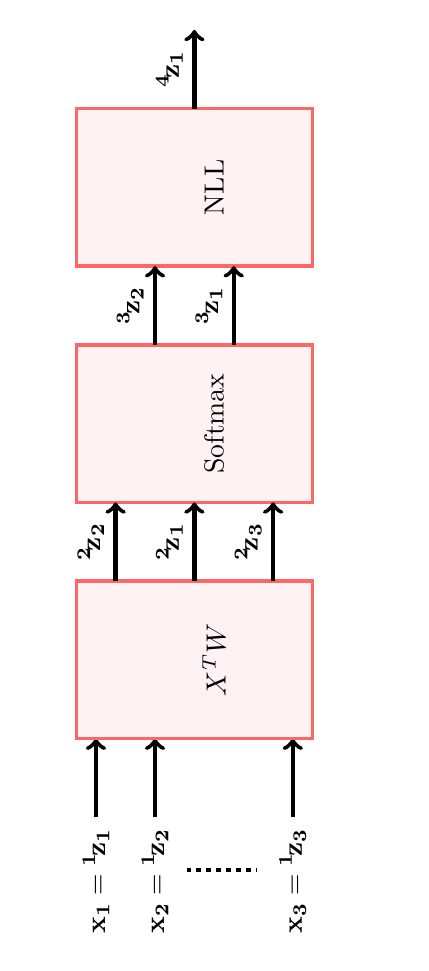
\begin{tikzpicture}[rotate=90]
    \node (B) at (3,0) {};
    \node (C) at (6,0) {};
    \node (D) at (9,0) {};

    \node (x1) at (1,3.5) {};
    \node (x2) at (1,2) {};
    \node (x3) at (1,0.5) {};
    \node (x4) at (1,-1) {};

    \draw[ultra thick, ->] (2,2.75) -> (3,2.75) node [pos=0,rotate=90,left,sloped] (TextNode) {$\mathbf{x_{1} = {}^{1}\!z_{1}}$};
    \draw[ultra thick, ->] (2,2) -> (3,2) node [pos=0,left,rotate=90,sloped] (TextNode) {$\mathbf{x_{2}={}^{1}\!{z_{2}}}$};
    \draw[ultra thick, ->] (2,0.25) -> (3,0.25) node [pos=0,left,sloped,rotate=90] (TextNode) {$\mathbf{x_{3}= {}^{1}\!z_{3}}$};
    \draw[ultra thick, dotted] (1.33,1.6) -- (1.33,0.7);


    \filldraw[color=red!60, fill=red!5, very thick,](B) rectangle +(2,3) node {};
    \draw (B)+(1,1.25) node [rotate=90]{$X^{T}W$};

    \filldraw[color=red!60, fill=red!5, very thick](C) rectangle +(2,3) node {};
    \draw (C)+(1,1.25) node [rotate=90]{Softmax};

    \filldraw[color=red!60, fill=red!5, very thick](D) rectangle +(2,3) node {};
    \draw (D)+(1,1.25) node [rotate=90]{NLL};


    \draw[ultra thick, ->] (5,1.5) -> (6,1.5) node [pos=0.5,rotate=90,above] (TextNode) {$\mathbf{{}^{2}\!z_{1}}$};
    \draw[ultra thick, ->] (5,2.5) -> (6,2.5) node [pos=0.5,rotate=90,above] (TextNode) {$\mathbf{{}^{2}\!z_{2}}$};
    \draw[ultra thick, ->] (5,0.5) -> (6,0.5) node [pos=0.5,rotate=90,above] (TextNode) {$\mathbf{{}^{2}\!z_{3}}$};

    \draw[ultra thick, ->] (8,1) -> (9,1) node [pos=0.5,rotate=90,above] (TextNode) {$\mathbf{{}^{3}\!z_{1}}$};
    \draw[ultra thick, ->] (8,2) -> (9,2) node [pos=0.5,rotate=90,above] (TextNode) {$\mathbf{{}^{3}\!z_{2}}$};

    \draw[ultra thick, ->] (11,1.5) -> (12,1.5) node [pos=0.5,rotate=90,above] (TextNode) {$\mathbf{{}^{4}\!z_{1}}$};


  \end{tikzpicture}
\end{centering}

\end{document}